\documentclass[../main.tex]{subfiles}

\begin{document}

Comparing Repour and Reqour with respect to scalability, there is no difference except one operation, and that is the alignment operation. The difference is shown in Figure \ref{fig:scalability}.

On the left side, we can see how the alignment operation works within Repour implementation: there are 2 pods\footnote{\url{https://docs.openshift.com/container-platform/4.17/rest_api/workloads_apis/pod-v1.html}} (inside PNC production cluster). The manipulator process itself (\textit{java -jar manipulator.jar}) is running directly inside one of the pods (depends which pod was picked to handle the request by Kubernetes built-in load-balancer\footnote{\url{https://docs.openshift.com/container-platform/4.17/rest_api/network_apis/service-v1.html}}). Since Repour is assigning asynchronous tasks to the asyncio event loop, there might be several running manipulator processes within the very same pod.

On the right side, we can see how alignment works within Reqour implementation: new Adjuster Job is being started for every new alignment (for further details, see \ref{subsec:alignment-design}).

\begin{figure}
  \begin{center}
    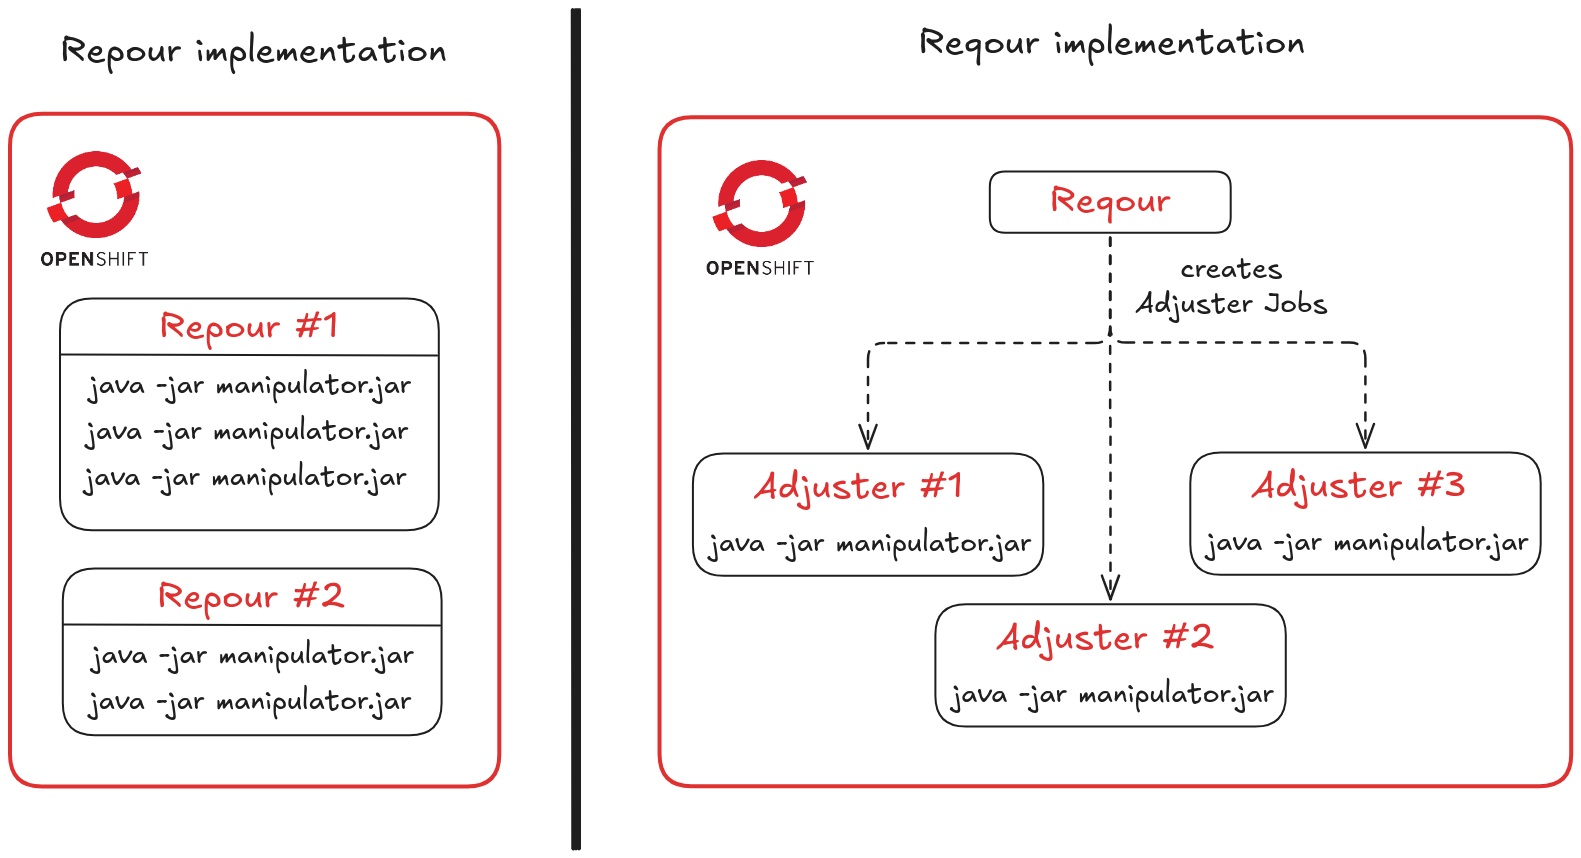
\includegraphics[width=\textwidth]{images/scalability.png}
  \end{center}
  \caption{Difference between Repour and Reqour alignment operation}
  \label{fig:scalability}
\end{figure}

\end{document}
